% move page numbers to top of page
\clearscrheadfoot            
\rohead[\pagemark]{\pagemark}
\lehead[\pagemark]{\pagemark}

% ------------------------------------------------------------------------------------------
\chapter{ICON standard level heights}
\label{appendix_levelheights}
% ------------------------------------------------------------------------------------------




% ------------------------------------------------------------------------------------------
\section{Level heights for zero topography height}
% ------------------------------------------------------------------------------------------

ICON standard \emph{half level} heights $z^{h0}$ are listed in
Table~\ref{tab:half_level_heights}.
%
Please note that these values correspond to the actual level heights only
at grid points with zero topography height, e.\,g.\ at ocean grid points.

If \emph{full level} heights $z^{f0}$ are required, these can be deduced as
follows:
%
Let $i$ denote the full level index for which the height is wanted. Then the full level 
height $z^{f0}_{i}$ is given by
\begin{align*}
 z^{f0}_{i} = \frac{ z^{h0}_{i} + z^{h0}_{i+1} }{2}.
\end{align*}
See Table~\ref{tab:full_level_heights} for a list of all full level heights of the operational
setup.


\begin{table}[p]
  \caption{Standard heights~$z_i^{h0}$ (i.e.\ for zero topography height) for all $91$ vertical 
           \underline{\emph{half levels}} of the global $13$ km domain and the $61$ vertical
	   half levels for the $6.5$ km EU nest.}
  \label{tab:half_level_heights}%
  \addtocounter{table}{-1} % we need this because we have a nested table-longtable environment

   \renewcommand{\baselinestretch}{1.00}\normalsize%
   \pgfkeys{/pgf/number format/set thousands separator={\,}}
   \pgfplotstableread{level_tables/vertical_levels_i.txt}{\loadedtable}\vspace*{0pt}%
   \pgfplotstabletypeset[ 
          begin table=\begin{longtable}, 
          end table=\end{longtable},
          columns={k,n,z,k,n,z,k,n,z},
          every  head row/.style={%
		  before row={\multicolumn{2}{>{\columncolor[gray]{.8}}c}{level index} & \multicolumn{2}{c}{height} &
		              \multicolumn{2}{>{\columncolor[gray]{.8}}c}{level index} & \multicolumn{2}{c}{height} &
		              \multicolumn{2}{>{\columncolor[gray]{.8}}c}{level index} & \multicolumn{2}{c}{height} \\%
	                     },
		  after row=\bottomrule,
	          },
          precision=2,
          font=\normalsize,
          columns/k/.style={column name=global     , column type=c, 
                            column type/.add={>{\columncolor[gray]{.8}}}{}},
          columns/n/.style={column name=EU nest    , column type=c, 
                            column type/.add={>{\columncolor[gray]{.8}}}{}},
          columns/z/.style={column name=$[m]$, fixed,dec sep align, zerofill,precision=3},
          display columns/0/.style={select equal part entry of={0}{3},string type},
          display columns/1/.style={select equal part entry of={0}{3},string type},
          display columns/2/.style={select equal part entry of={0}{3}},
          display columns/3/.style={select equal part entry of={1}{3},string type},
          display columns/4/.style={select equal part entry of={1}{3},string type},
          display columns/5/.style={select equal part entry of={1}{3}},
          display columns/6/.style={select equal part entry of={2}{3},string type},
          display columns/7/.style={select equal part entry of={2}{3},string type},
          display columns/8/.style={select equal part entry of={2}{3}}
                        ] {\loadedtable}

\end{table}

\begin{table}[p]
  \caption{Standard heights~$z_i^{f0}$ (i.e.\ for zero topography height) for all $90$ vertical 
           \underline{\emph{full levels}} of the global $13$ km domain.}
  \label{tab:full_level_heights}%
  \addtocounter{table}{-1} % we need this because we have a nested table-longtable environment

   \definecolor{maroon}{cmyk}{0,0.87,0.68,0.32}
   \renewcommand{\baselinestretch}{1.00}\normalsize%
   \pgfkeys{/pgf/number format/set thousands separator={\,}}
   \pgfplotstableread{level_tables/vertical_full_levels_i.txt}{\loadedtable}\vspace*{0pt}%
   \pgfplotstabletypeset[ 
          begin table=\begin{longtable}, 
          end table=\end{longtable},
          columns={k,z,k,z,k,z},
          every  head row/.style={after row={\hline}},
          precision=2,
          font=\normalsize,
          columns/k/.style={column name=level index, column type=c, 
                            column type/.add={>{\columncolor{maroon!15}}}{}},
          columns/z/.style={column name=height $[m]$, fixed,dec sep align, zerofill,precision=3},
          display columns/0/.style={select equal part entry of={0}{3},string type},
          display columns/1/.style={select equal part entry of={0}{3}},
          display columns/2/.style={select equal part entry of={1}{3},string type},
          display columns/3/.style={select equal part entry of={1}{3}},
          display columns/4/.style={select equal part entry of={2}{3},string type},
          display columns/5/.style={select equal part entry of={2}{3}},
                        ] {\loadedtable}

\end{table}


% ------------------------------------------------------------------------------------------
\section{Non-zero topography heights}
% ------------------------------------------------------------------------------------------

The prerequisite ''zero topography height'' is seldom met in real
applications.
Instead the user has to compute the model level height for each grid
point separately.
To this end the invariant fields \texttt{HSURF} and \texttt{HHL} are
provided where \texttt{HHL} is the geometric height of model half
levels above sea level.
The level height above ground can therefore be computed by the
following formula:
\begin{align*}
  z^{h}_{i}(x) &= \texttt{HHL}(x) - \texttt{HSURF}(x) \\[0.5em]
  %
  z^{f}_{i}(x) &= \frac{ z^{h}_{i}(x) + z^{h}_{i+1}(x) }{2} 
\end{align*}

\begin{table}[p]
  \caption{Height above ground~$z_i^h(x)$ (half levels) for the grid point with maximum topography height
    in the operational setup R03B07, 13\,km spatial resolution.}
  
  \vspace*{2em}
  \begin{tikzpicture}
    \node[draw,rectangle] (0,0) {
      \begin{minipage}{0.96\textwidth}
        \vspace*{3em}%
        \begin{tabbing}     
          \hspace*{3em}%
          \begin{minipage}[b]{0.55\textwidth}\vspace*{0em}%
            \underline{\textbf{Example: Height above ground \texttt{HHL} - \texttt{HSURF}}}\\[1em]
            Location with max.\ surface height\\    
            \begin{tabbing}
              \texttt{CLON}/\texttt{CLAT}   \== 88.180 / 27.938          \\[0.5em]
              \texttt{HSURF}                \>=   6425.974 m
            \end{tabbing}
          \end{minipage}
          \=\hspace*{3.0em}%
          \begin{minipage}[c]{0.25\textwidth}\vspace*{-8em}%
            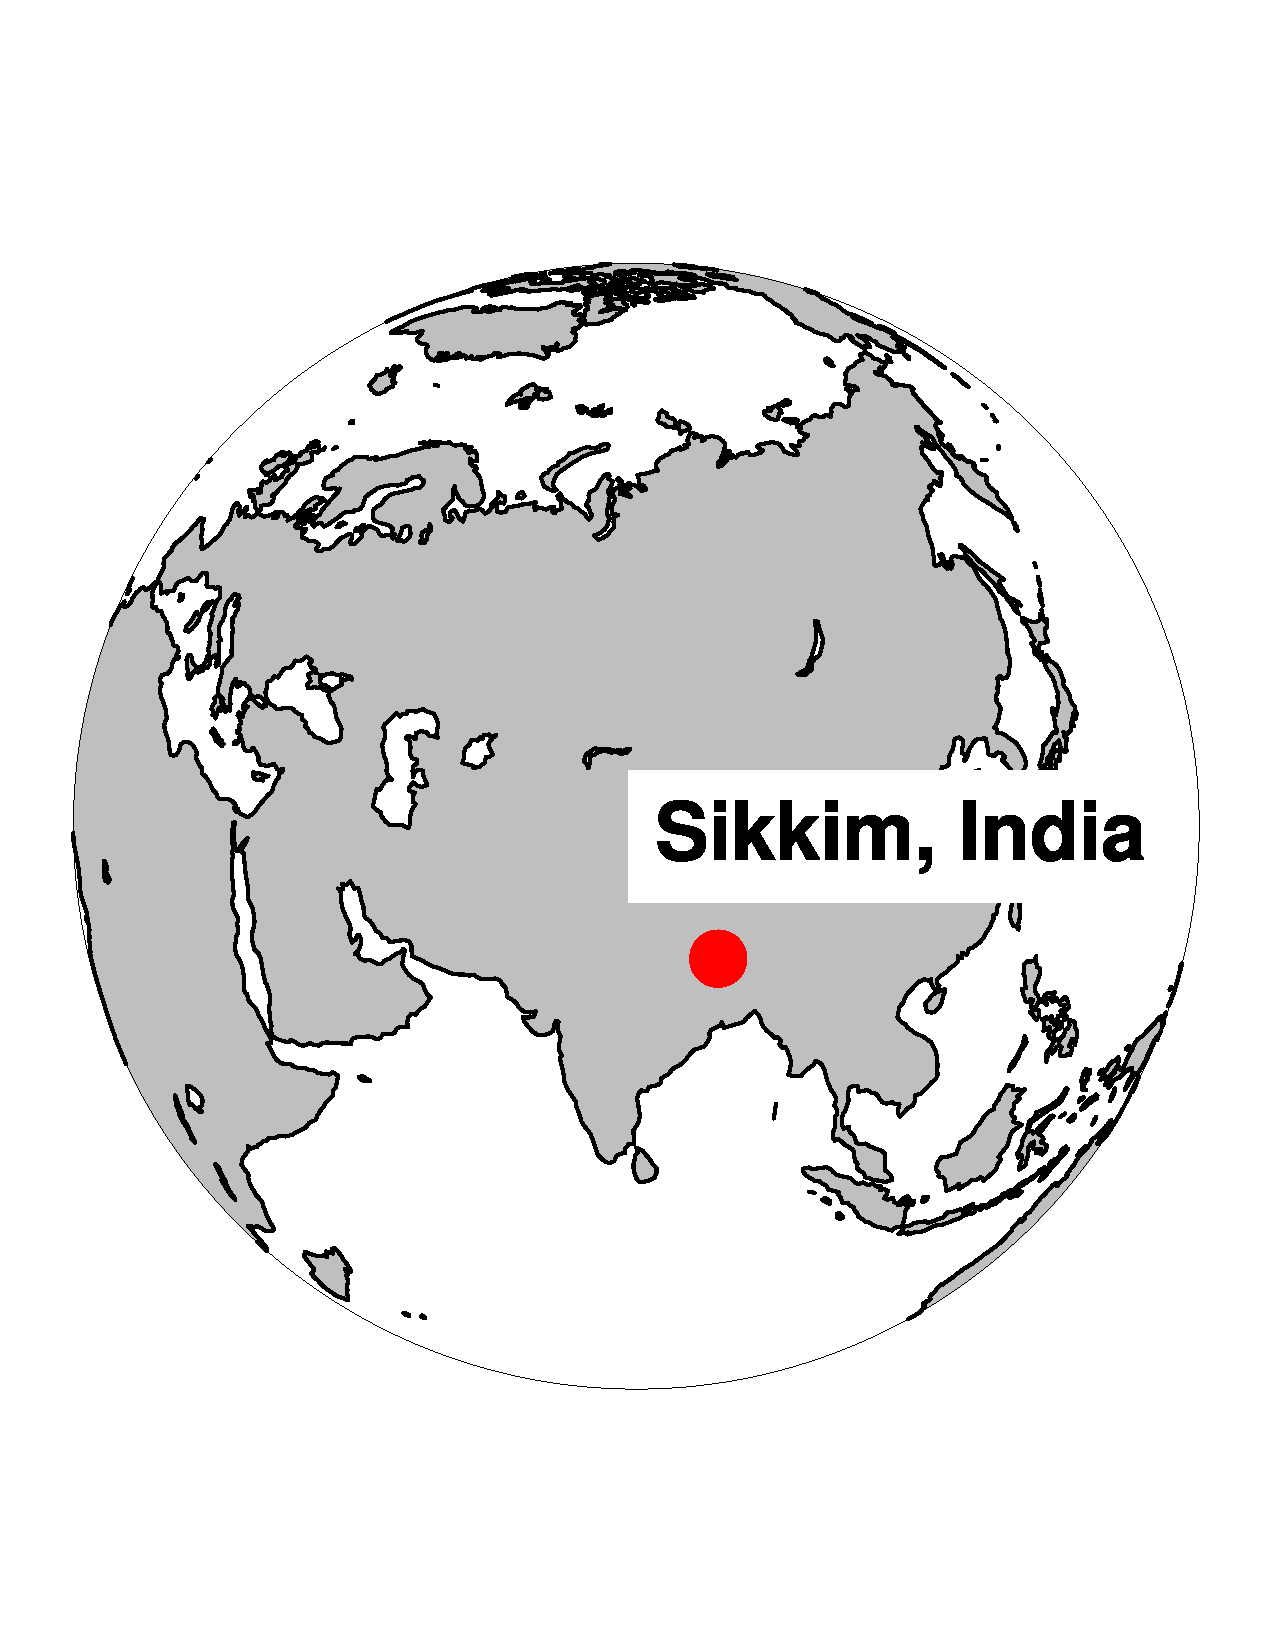
\includegraphics[width=\textwidth]{pics/plot_maxhsurf.pdf}
          \end{minipage}
        \end{tabbing}

        \addtocounter{table}{-1} % we need this because we have a nested table-longtable environment
        \definecolor{bggreen}{cmyk}{0.38, 0.00, 0.25, 0.16 }
        \renewcommand{\baselinestretch}{1.00}\normalsize%
        \pgfkeys{/pgf/number format/set thousands separator={\,}}
        \pgfplotstableread{level_tables/vertical_half_levels_maxheight_i.txt}{\loadedtable}\vspace*{0pt}%
        \pgfplotstabletypeset[ 
        begin table=\begin{longtable}, 
          end table=\end{longtable},
        columns={k,z,k,z,k,z,k,z},
        every  head row/.style={after row={\hline}},
        precision=2,
        font=\normalsize,
        columns/k/.style={column name=level idx., column type=c, 
          column type/.add={>{\columncolor{bggreen!15}}}{}},
        columns/z/.style={column name=height $[m]$, fixed,dec sep align, zerofill,precision=3},
        display columns/0/.style={select equal part entry of={0}{4},string type},
        display columns/1/.style={select equal part entry of={0}{4}},
        display columns/2/.style={select equal part entry of={1}{4},string type},
        display columns/3/.style={select equal part entry of={1}{4}},
        display columns/4/.style={select equal part entry of={2}{4},string type},
        display columns/5/.style={select equal part entry of={2}{4}},
        display columns/6/.style={select equal part entry of={3}{4},string type},
        display columns/7/.style={select equal part entry of={3}{4}},
        ] {\loadedtable}
      \end{minipage}
    };
  \end{tikzpicture}
\end{table}


\begin{table}[p]
  \caption{Height above ground~$z_i^f(x)$ (full levels) for the grid point with maximum topography height
    in the operational setup R03B07, 13\,km spatial resolution.}
  
  \vspace*{2em}
  \begin{tikzpicture}
    \node[draw,rectangle] (0,0) {
      \begin{minipage}{0.96\textwidth}
        \vspace*{3em}%
        \begin{tabbing}     
          \hspace*{3em}%
          \begin{minipage}[b]{0.55\textwidth}\vspace*{0em}%
            \underline{\textbf{Example: Height above ground, full levels}}\\[1em]
            Location with max.\ surface height\\    
            \begin{tabbing}
              \texttt{CLON}/\texttt{CLAT}   \== 88.180 / 27.938          \\[0.5em]
              \texttt{HSURF}                \>=   6425.974 m
            \end{tabbing}
          \end{minipage}
          \=\hspace*{3.0em}%
          \begin{minipage}[c]{0.25\textwidth}\vspace*{-8em}%
            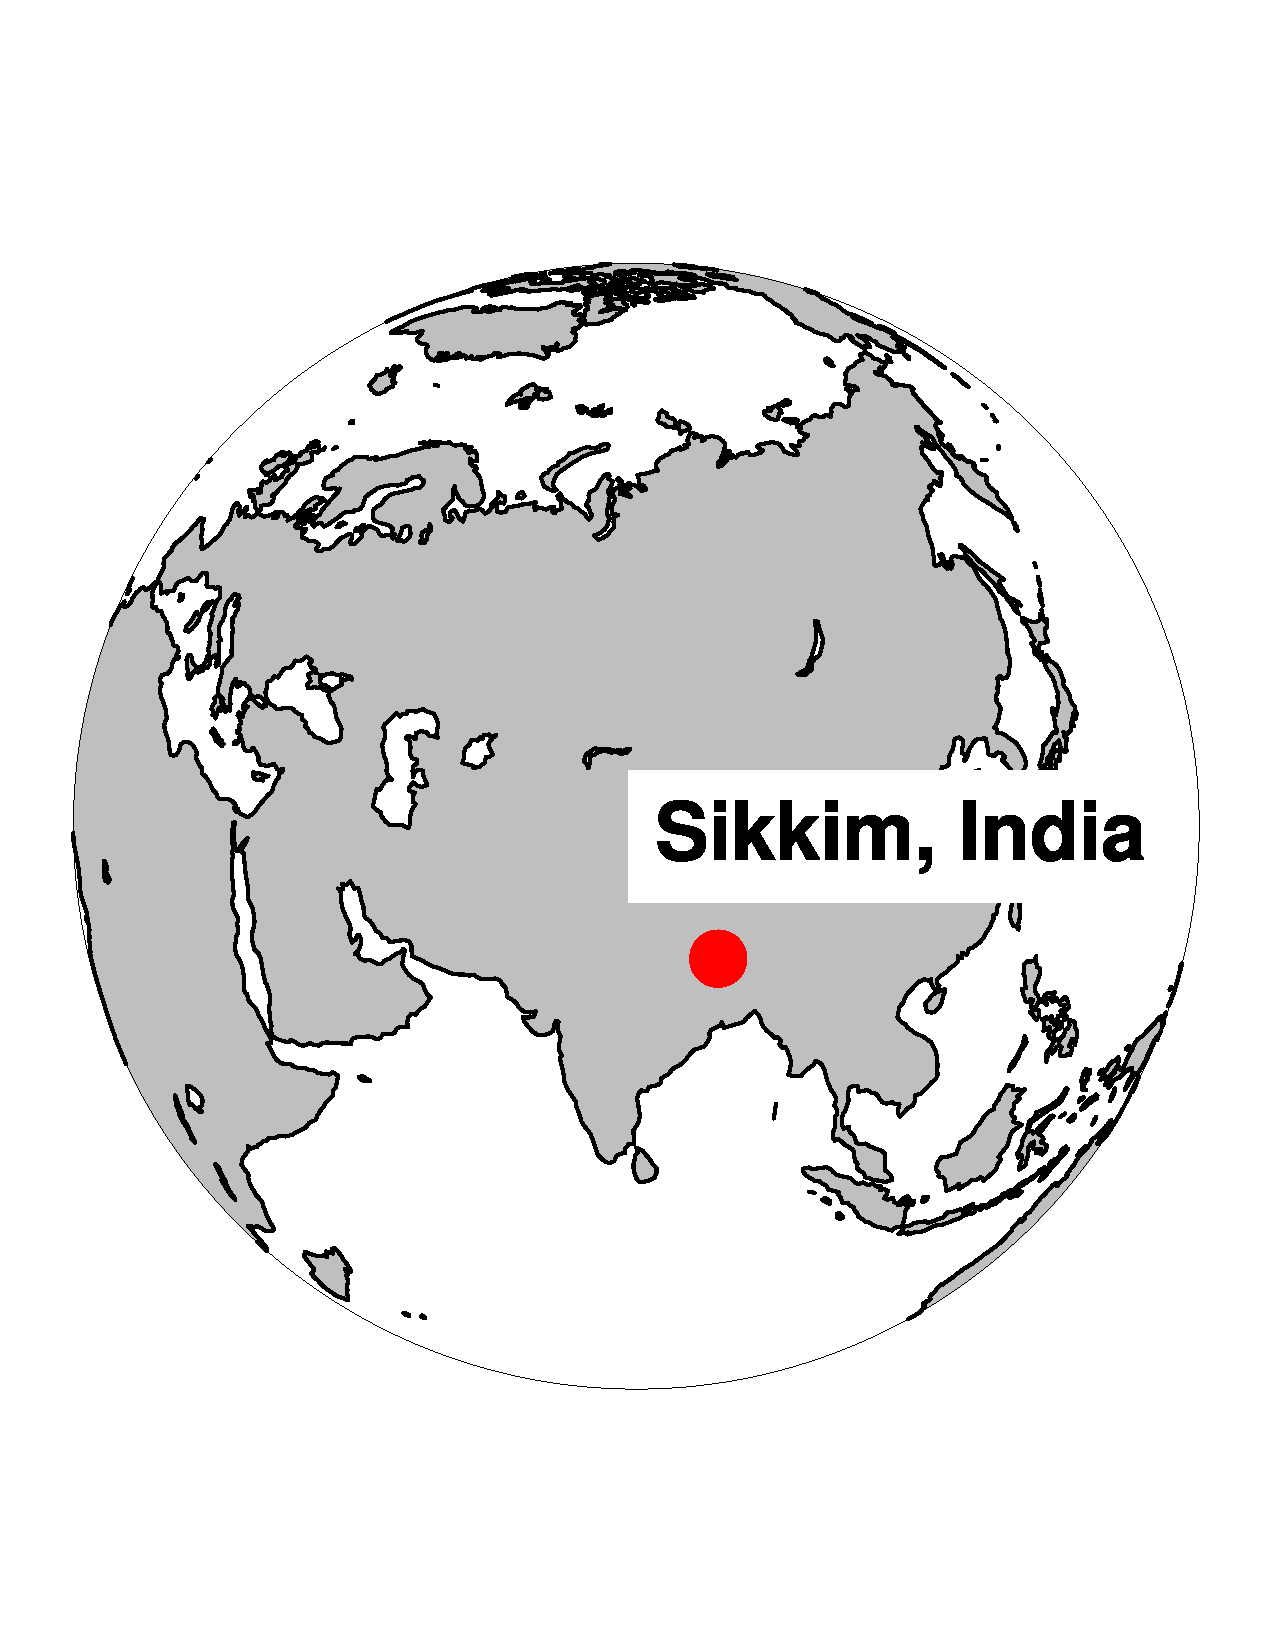
\includegraphics[width=\textwidth]{pics/plot_maxhsurf.pdf}
          \end{minipage}
        \end{tabbing}

        \addtocounter{table}{-1} % we need this because we have a nested table-longtable environment
        \definecolor{bgblue}{cmyk}{ 0.53, 0.20, 0.00, 0.27}
        \renewcommand{\baselinestretch}{1.00}\normalsize%
        \pgfkeys{/pgf/number format/set thousands separator={\,}}
        \pgfplotstableread{level_tables/vertical_full_levels_maxheight_i.txt}{\loadedtable}\vspace*{0pt}%
        \pgfplotstabletypeset[ 
        begin table=\begin{longtable}, 
          end table=\end{longtable},
        columns={k,z,k,z,k,z,k,z},
        every  head row/.style={after row={\hline}},
        precision=2,
        font=\normalsize,
        columns/k/.style={column name=level idx., column type=c, 
          column type/.add={>{\columncolor{bgblue!15}}}{}},
        columns/z/.style={column name=height $[m]$, fixed,dec sep align, zerofill,precision=3},
        display columns/0/.style={select equal part entry of={0}{4},string type},
        display columns/1/.style={select equal part entry of={0}{4}},
        display columns/2/.style={select equal part entry of={1}{4},string type},
        display columns/3/.style={select equal part entry of={1}{4}},
        display columns/4/.style={select equal part entry of={2}{4},string type},
        display columns/5/.style={select equal part entry of={2}{4}},
        display columns/6/.style={select equal part entry of={3}{4},string type},
        display columns/7/.style={select equal part entry of={3}{4}},
        ] {\loadedtable}
      \end{minipage}
    };
  \end{tikzpicture}
\end{table}
